% Chapter 3

\chapter{Experimental setup} % Main chapter title

\label{Chapter3} % For referencing the chapter elsewhere, use \ref{Chapter3}


%----------------------------------------------------------------------------------------

\section{Introduction}
The majority of prediction tools are based on the assumption that it is the miRNA seed region that contains almost all the important interactions between a miRNA and its target and their focus is on these canonical sites.

In this thesis we aim at using deep learning techniques to investigate the role of those non-canonical sites and pairing beyond the canonical seed region in miRNA targets. Recent increases in computational power have permitted the rise of methods that can dispense with human-crafted features, making it possible to deal directly with raw data and autonomously learn and identify patterns to appropriately represent it. In particular, deep learning has been shown to be an effective method for classification tasks in domains with complex feature representation \cite{dl}.

DL has already been applied to the miRNA target prediction problem. Cheng et al. \cite{mirtdl} used convolutional neural networks to analyze matrices of miRNA:site features, but the selected features were still human-crafted descriptors and thus the method faces similar problems as rule-based and ML approaches. A more recent work, DeepTarget \cite{deep_target}, relied on recurrent neural networks to identify potential binding sites and assess their functionality. However this work is still oriented to the identification of canonical sites and relies on a limited small data set for the training phase. Another approach using DL is DeepMirTarSdA \cite{deep_mirtar}, that explore the use of stacked de-noising auto-encoders (SdA) to predict human miRNA-targets at the site level, but the network obtained is huge and the small availability of input data (about 8000 samples between positives and negatives) results in a model that performs well on the data being used but generalizes quite poorly. 

In this thesis we present DeepMiRNA, a miRNA target prediction tool that attempts to take advantage of the learning capacity of a neural network to extract abstract patterns from raw input data. Unfortunately, to the best of our knowledge, there is no suitable raw-data representational method for miRNA-target prediction. This is very likely the consequence of the very small quantity of validated data available for this task. For this reason, rather than making assumption about suitable descriptor, we created a set of rules to help finding the best candidate binding sites leaving the classification decision to the neural network (see CSSM in the next section).

More precisely, DeepMiRNA scans the 3'UTR of the gene identifying potential target sites according to the chosen rules. It then uses the previously trained network to identify the relevant patterns by directly examining the whole mature miRNA transcript, rather than focusing on the seed region and analyzing precomputed descriptors.

\section{Materials and methods}
Two of the fundamental properties in deep neural network theory states that:

\begin{enumerate}
	\item with sufficient data samples and a correct network design a NN can approximate any mathematical function
	\item a NN has the capacity to automatically learn the relevant features of complex data structures by means of its hidden layers \cite{dl}
\end{enumerate}

For these reasons, in our approach we sought to minimize potential biases introduced by handcrafted features by working  with the miRNA and the mRNA transcripts, feeding them directly to the neural network.

The DeepMiRNA working pipeline for the identification of functional targets for miRNAs can be summarized as follows (Figure \ref{fig:pipeline}: a 30-nucleotide sliding window with stride of 5 nucleotides is used to scan the 3'UTR of a given gene. Both values (size and stride) has been empirically computed during the training stage (see the results section for more informations). For each mRNA 30-nucleotide long subsequence, the VIENNA RNACofold package \cite{vienna_rna} is used to compute the stability of the binding between the miRNA transcript and the fragment. If the computed value is below a predetermined threshold, the primary structure of the mRNA and the miRNA are examined to see if the criteria defined by the candidate site selection rules (CSSR) are met. If so, the duplex is vectorized and fed into the network for classification. The prediction is then further refined using an a posteriori filter that computes the site accessibility of the mRNA region surrounding the predicted binding site. This last step has revealed an important role in false positive reduction and it's used only for positive predictions.

\begin{figure}[hbt!]
	\centering
	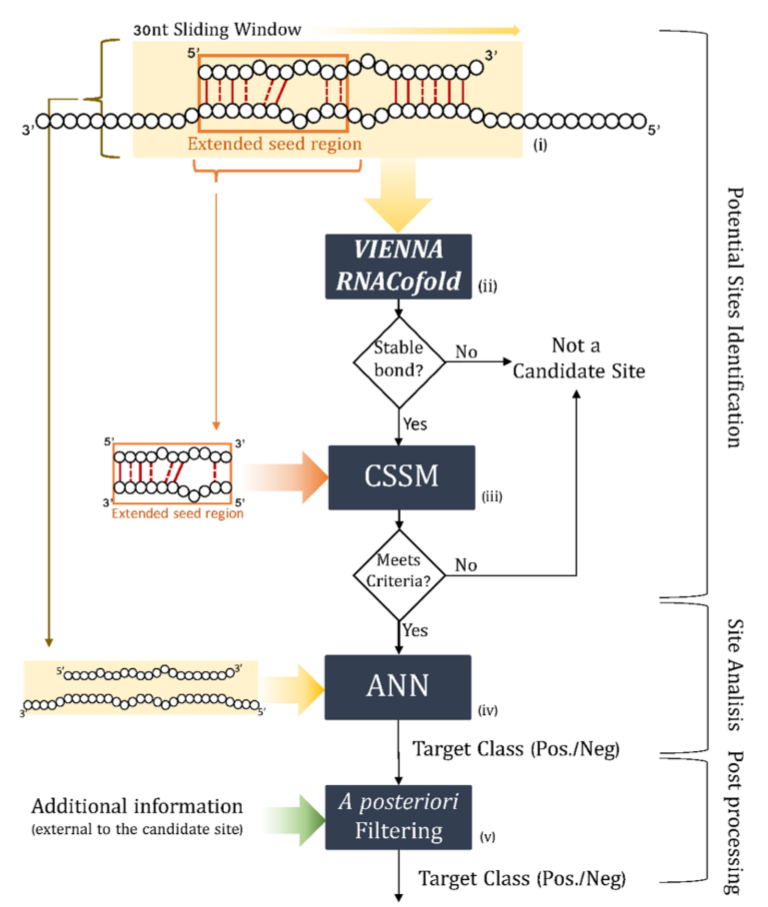
\includegraphics[width=0.8\textwidth]{Figures/pipeline}
	\caption{\textbf{DeepMiRNA pipeline}. (i) a 30nt sliding window with a 5nt step is used to scan the gene transcript; (ii) The Vienna Cofold software is used to compute the binding stability; (iii) if the bond is predicted to be stable a partial complementarity according to the rules defined in the CSSR is verified; (iv) if all previous checks passed the duplex is fed to the NN for prediction; (v) for positive predictions a filter is used to compute the site accessibility of the miRNA: if the energy needed to access the site is above a certain threshold the prediction is changed to negative.}
	\label{fig:pipeline}
\end{figure}

\subsection{Data preprocessing}
A key factor for successful application of any Machine Learning technique and one of the most important aspect to consider before feeding the network with data is how we prepare the input data and the targets. The main purpose is to have a sufficiently variable and representative dataset that allows the model to generalize well on new and unseen examples. This phase is probably the most important together with the network design as it's crucial for achieving good performances. 

The two main aspects to consider during this process are the following:

\begin{enumerate} 
	\item use suitable techniques to make the data more amenable for the NN: this includes vectorization, normalization and handling of missing values. 
	\item find comprehensive and validated data representative of the classification problem. 
\end{enumerate} 

\subsubsection{vectorization}
In order to be accepted by the neural network all inputs must be tensors, that is they must be expressed by numerical arrays with suitable shape and dimension. The process to encode categorical data, in our case the transcript sequences, into tensor is called \emph{vectorization}. In this thesis we actually employed two different techniques for this operation: 

\begin{itemize} 
	\item one hot encoding of the sequences \cite{onehotencode}. 
	\item sequence embedding using a Word2Vec approach \cite{word2vec}. 
\end{itemize}

One hot encoding is a process by which categorical data such as strings are converted into binary vectors. In our case, each nucleotide is translated to a binary vector of size 4, corresponding to the four possible nucleotide values as described in Table \ref{tab:ohe} 

\begin{table}[!b]
	\caption{One Hot encoding of a nucleotide.}
	\label{tab:ohe}
	\centering
	\begin{tabular}{l l}
		\toprule
		\tabhead{Nucleotide} & \tabhead{Encoding} \\
		\midrule
		A & [1, 0, 0, 0]\\
		C & [0, 1, 0, 0]\\
		G & [0, 0, 1, 0]\\
		U or T & [0, 0, 0, 1]\\
		Empty & [0, 0, 0, 0]\\
		\bottomrule
	\end{tabular}
\end{table}

The main problem using this method is that not all duplexes have the same size. This is in particular due to the different miRNA's transcript length (ranges from 18 to 30), The network, instead, requires that all inputs have the same shape. Hence, in order to meet this requirement, any miRNA sequence is padded with 'empty' letters to reach the maximum size (in this case 30). Regarding the site transcript, each fragment has size 40: 30 corresponding to the window size plus 5 additional nucleotides upstream and downstream. These additional nucleotides seek to capture any influence that the flanking sequence may exert on the target \cite{conserved_pairing}. With these adjustments each duplex is represented by a binary vector of (fixed) size 280.

The second vectorization method uses a Word2Vec approach. Word2Vec \cite{word2vec} is a Natural Language Processing (NLP) methodology to map words into numeric vectors based on their context. Being the context defined as the words surrounding the word to encode. For DNA sequences, however, there is no clear definition for words, so usually a k-mer (that is a set of $k$ continuous nucleotides)is used to define a word (see Figure \ref{fig:dna2vec}). Therefore, in case of biological sequences the context is defined as the set of $n$ adjacent k-mers (being $n$ a parameter to validate). For this thesis use the software available at \url{https://github.com/pnpnpn/dna2vec} to train the model used to encode the k-mers. This encoding has two important advantages compared to one hot encoding:

\begin{enumerate}
	\item each k-mer of length comprised between 3 and 8 is mapped to an equal size vector of size 100.
	\item similar k-mers are mapped to close points in the features space according to a specific distance metric (usually Euclidean distance).
\end{enumerate}

In our case each variable lenght miRNA sequence has been split into 4 different size k-mers each mapped into a 100-dimension vector, while each fixed size site transcript (plus the flanking nucleotides) has been split into 5 8-mers. This way each duplex is mapped into a $9x100$ matrix obtained concatenating the resulting 9 vectors. It's important to note that this vectorization requires a different design and implementation of the neural network to use as we will describe in the next section.

\begin{figure}[hbt!]
	\centering
	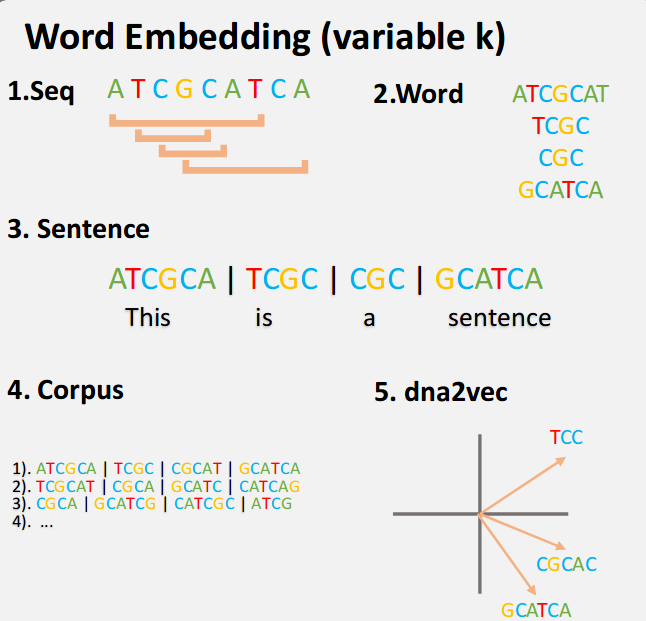
\includegraphics[width=0.7\textwidth, height=0.3\textheight]{Figures/dna2vec}
	\caption{\textbf{Dna2Vec mapping example using different length k-mers}}
	\label{fig:dna2vec}
\end{figure}

\subsubsection{normalization and missing values}
Another crucial part of data preprocessing concerns their normalization. In general, it's not safe to feed the network with data that takes relatively large values or that are heterogeneous (i.e have very different values ranges). In our case, however, the vectorization process guarantees that the numerical values resulting from the encoding are both small and homogeneous. Regarding missing or incomplete data, we found a very small quantity  of them in the datasets retrieved, hence we simply decided to discard them.  

\subsection{Dataset preparation}